\documentclass{standalone}

\usepackage{tikz}
\usetikzlibrary{
    shapes,
    positioning,
    fit,
}

\tikzset{
    double distance=2pt,
    node distance=1.5cm,
    entity/.style={rectangle, draw, text centered, minimum height=1cm, minimum width=2.5cm, align=center},
    attribute/.style={ellipse, draw, text centered, minimum height=0.7cm, minimum width=1.5cm, align=center},
    relation/.style={diamond, draw, text centered, minimum height=0.5cm, minimum width=1.5cm, align=center, aspect=2},
    spec/.style={circle, draw, text centered, minimum width=0.4, align=center},
    cardinality/.style={font=\small},
    multivaluedattribute/.style={attribute, double},
    agg/.style={draw, inner sep=10pt},
}

\begin{document}

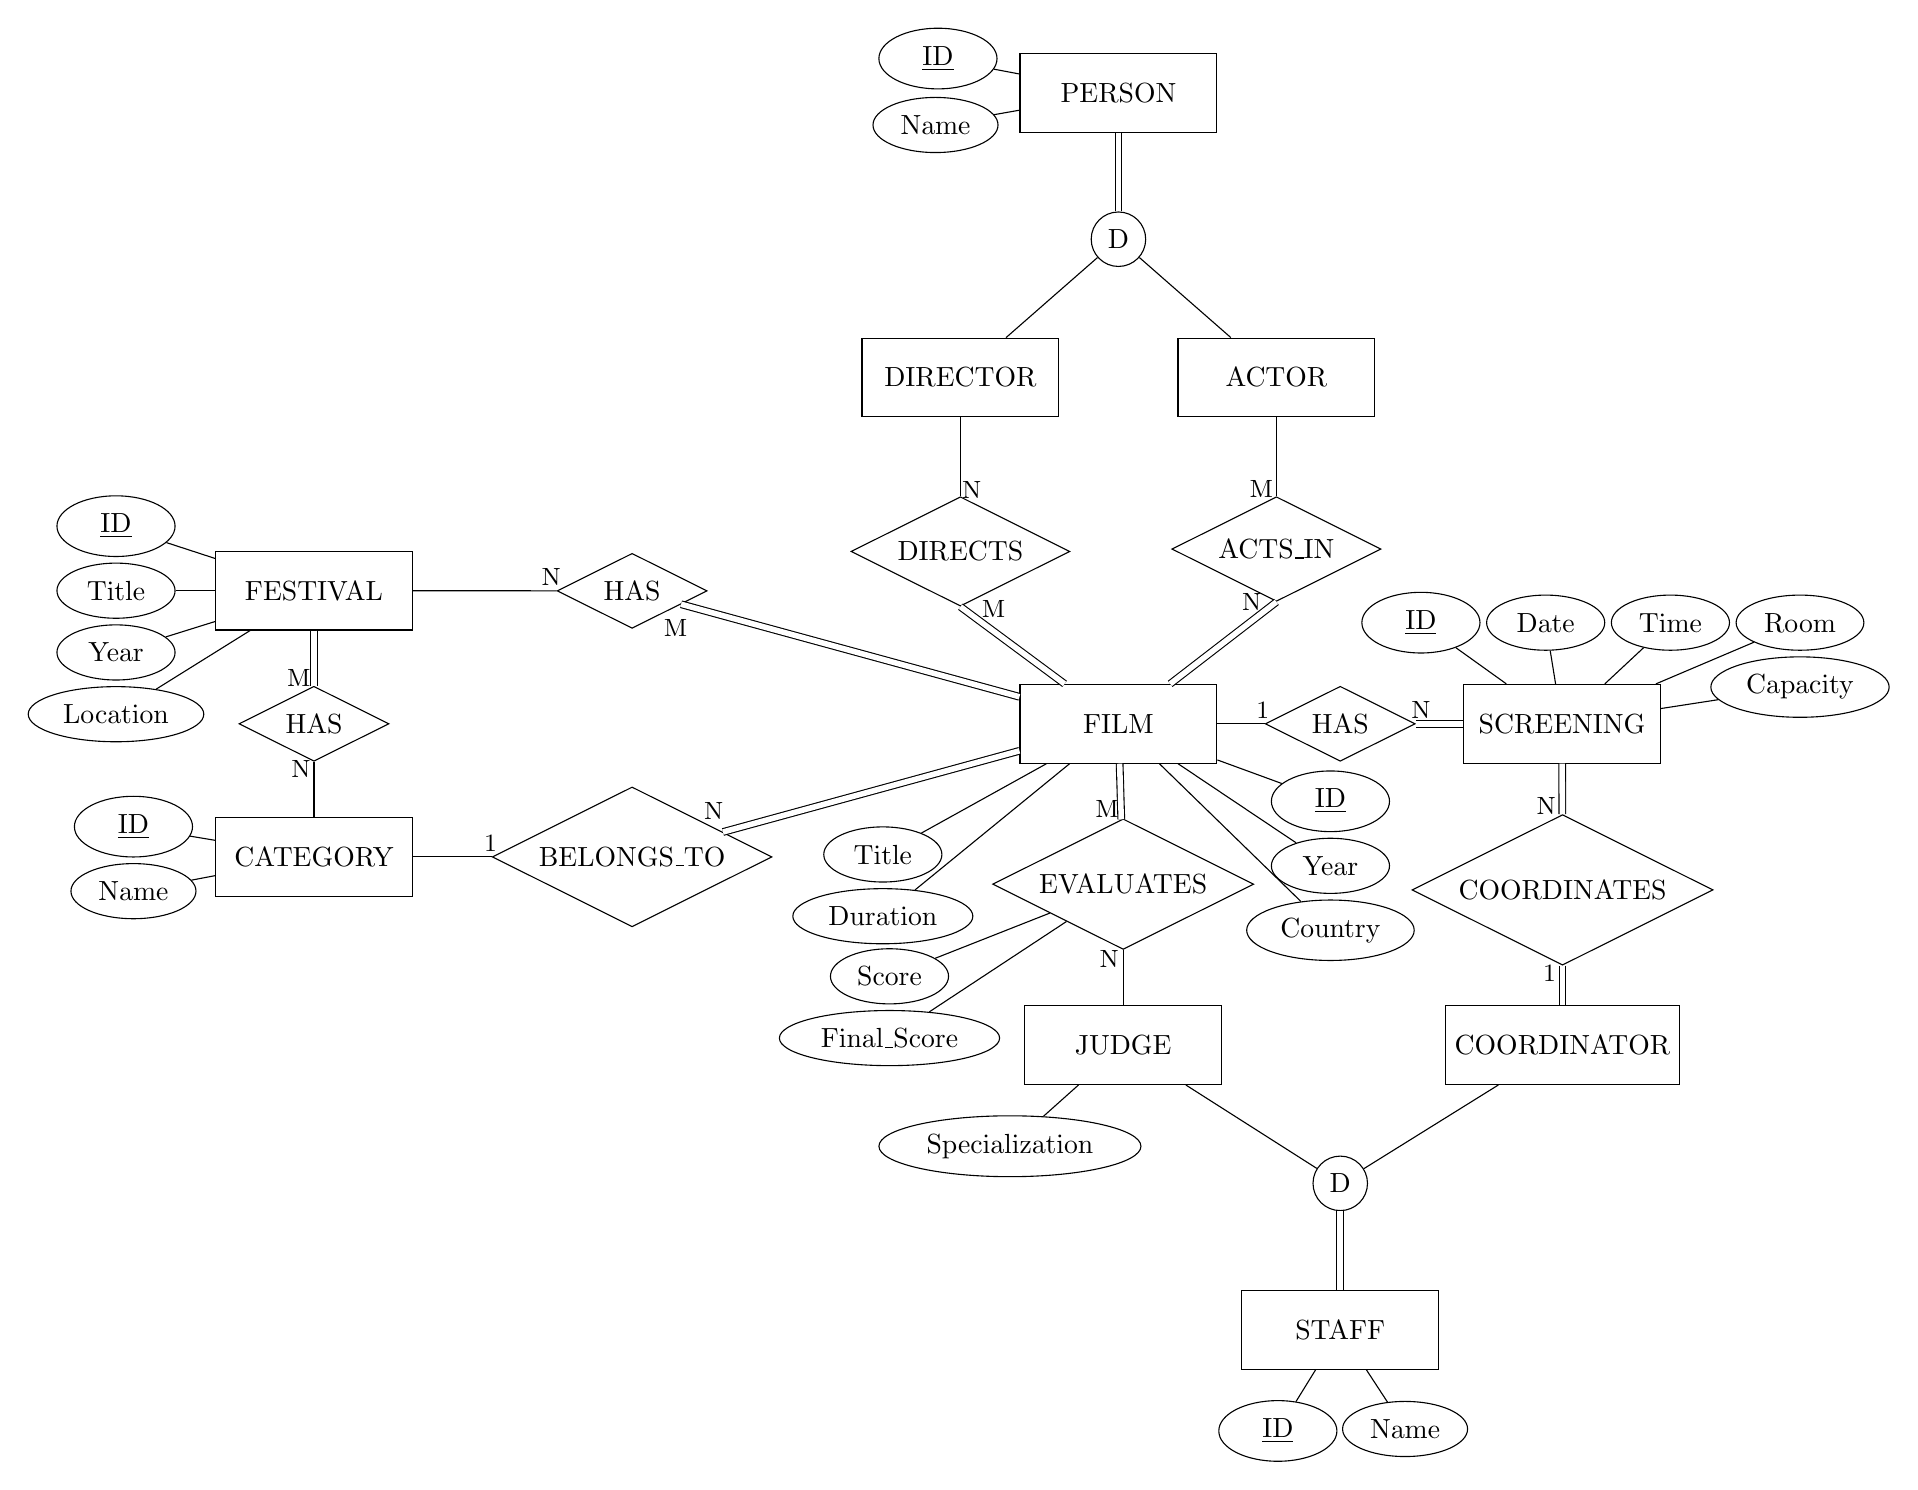
\begin{tikzpicture}
    \node[entity] (festival) {FESTIVAL};

    \node[attribute, left=5mm of festival] (ftitle) {Title};
    \node[attribute, above=2pt of ftitle] (fid) {\underline{ID}};
    \node[attribute, below=2pt of ftitle] (fyear) {Year};
    \node[attribute, below=2pt of fyear] (flocation) {Location};

    \node[relation, below=7mm of festival] (fest_has) {HAS};
    \node[cardinality, above left=0.3em and -1.6em of fest_has] {M};
    \node[cardinality, below left=0.3em and -1.6em of fest_has] {N};

    \node[entity, below=7mm of fest_has] (category) {CATEGORY};

    \node[attribute, above left=-4mm and 5mm of category] (cid) {\underline{ID}};
    \node[attribute, below=2pt of cid] (cname) {Name};

    \node[relation, right=1cm of category] (belongs_to) {BELONGS\_TO};
    \node[cardinality, above right=-1mm and -1mm of belongs_to] {N};
    \node[cardinality, above left=-5mm and 7mm of belongs_to] {1};

    \node[entity, right= 8cm of fest_has] (film) {FILM};

    \node[attribute, below right=2mm and 9mm of film] (filmid) {\underline{ID}};
    \node[attribute, below left=9mm and 12mm of film] (filmtitle) {Title};
    \node[attribute, below=2pt of filmtitle] (filmdur) {Duration};
    \node[attribute, below=2pt of filmid] (filmyear) {Year};
    \node[attribute, below=2pt of filmyear] (filmcountry) {Country};

    \node[entity, above=7cm of film] (person) {PERSON};

    \node[attribute, above left=-3.5mm and 5mm of person] (pid) {\underline{ID}};
    \node[attribute, below left=-3.5mm and 5mm of person] (pname) {Name};

    \node[spec, below=1cm of person] (person_spec) {D};
    \node[entity, below left=1cm and 0.5cm of person_spec] (director) {DIRECTOR};
    \node[entity, below right=1cm and 0.5cm of person_spec] (actor) {ACTOR};

    \node[relation, below=1cm of director] (directs) {DIRECTS};
    \node[cardinality, below right=1.5mm and -5.5mm of directs] {M};
    \node[cardinality, above right=2mm and -8mm of directs] {N};

    \node[relation, below=1cm of actor] (acts_in) {ACTS\_IN};
    \node[cardinality, above left=2mm and -7.5mm of acts_in] {M};
    \node[cardinality, below left=1mm and -6mm of acts_in] {N};

    \node[relation, above=2cm of belongs_to] (has_film) {HAS};
    \node[cardinality, above left=-3mm and 3mm of has_film] {N};
    \node[cardinality, below right=0mm and -2mm of has_film] {M};

    \node[relation, right=6mm of film] (film_has) {HAS};
    \node[cardinality, above left=-3mm and 3mm of film_has] {1};
    \node[cardinality, above right=-3mm and 3mm of film_has] {N};

    \node[spec, below=5cm of film_has] (staff_spec) {D};

    \node[entity, below=1cm of staff_spec] (staff) {STAFF};
    \node[attribute, below left=5mm and -1cm of staff] (sid) {\underline{ID}};
    \node[attribute, below right=5mm and -1cm of staff] (sname) {Name};

    \node[entity, above left=1cm and 12.5mm of staff_spec] (judge) {JUDGE};

    \node[attribute, below left=0.5cm and -1cm of judge] (specialization) {Specialization};

    \node[entity, above right=1cm and 10.8mm of staff_spec] (coordinator) {COORDINATOR};

    \node[entity, right=6mm of film_has] (screening) {SCREENING};

    \node[attribute, above left=5mm and 0mm of screening] (scid) {\underline{ID}};
    \node[attribute, right=2pt of scid] (scdate) {Date};
    \node[attribute, right=2pt of scdate] (sctime) {Time};
    \node[attribute, right=2pt of sctime] (scroom) {Room};
    \node[attribute, below=2pt of scroom] (sccap) {Capacity};

    \node[relation, above=5mm of coordinator] (coordinates) {COORDINATES};
    \node[cardinality, above left=3.5mm and -1cm of coordinates] {N};
    \node[cardinality, below left=3.5mm and -1cm of coordinates] {1};

    \node[relation, above=7mm of judge] (evaluates) {EVALUATES};
    \node[cardinality, above left=3mm and -9mm of evaluates] {M};
    \node[cardinality, below left=3mm and -9mm of evaluates] {N};

    \node[attribute, below left=5mm and 16mm of evaluates] (eval_score) {Score};
    \node[attribute, below=2pt of eval_score] (eval_final) {Final\_Score};

    % ===== DRAW ALL CONNECTIONS =====
    \draw (festival) -- (fid);
    \draw (festival) -- (ftitle);
    \draw (festival) -- (fyear);
    \draw (festival) -- (flocation);
    \draw[double] (festival) -- (fest_has);
    \draw (fest_has) -- (category);
    \draw (festival) -- (has_film);
    \draw[double] (has_film) -- (film);

    \draw (category) -- (cid);
    \draw (category) -- (cname);
    \draw (category) -- (belongs_to);
    \draw[double] (belongs_to) -- (film);

    \draw (film) -- (filmid);
    \draw (film) -- (filmtitle);
    \draw (film) -- (filmdur);
    \draw (film) -- (filmyear);
    \draw (film) -- (filmcountry);

    \draw (person) -- (pid);
    \draw (person) -- (pname);
    \draw[double] (person) -- (person_spec);
    \draw (person_spec) -- (director);
    \draw (person_spec) -- (actor);

    \draw (director) -- (directs);
    \draw[double] (directs.south) -- (film);

    \draw (actor) -- (acts_in);
    \draw[double] (acts_in.south) -- (film);

    \draw (film) -- (film_has);
    \draw[double] (film_has) -- (screening);

    \draw (screening) -- (scid);
    \draw (screening) -- (scdate);
    \draw (screening) -- (sctime);
    \draw (screening) -- (scroom);
    \draw (screening) -- (sccap);

    \draw[double] (screening) -- (coordinates);
    \draw[double] (coordinates) -- (coordinator);

    \draw (staff) -- (sid);
    \draw (staff) -- (sname);

    \draw (judge) -- (specialization);
    \draw (judge) -- (staff_spec);
    \draw (staff_spec) -- (coordinator);
    \draw[double] (staff_spec) -- (staff);

    \draw (judge) -- (evaluates);
    \draw[double] (evaluates) -- (film);
    \draw (evaluates) -- (eval_score);
    \draw (evaluates) -- (eval_final);

\end{tikzpicture}
\end{document}
